\documentclass[conference]{IEEEtran}
\usepackage{amsmath}
\usepackage{newtxtext}
\usepackage{newtxmath}
\usepackage{graphicx}

\graphicspath{{figs/}}

\begin{document}

\title{Preserving Hamiltonian Symmetry on Parallel Hardware:\\
Deterministic Reductions and Mixed-Precision Acceleration\\in GPU Symplectic Integration}

\author{\IEEEauthorblockN{Utkarsh Joshi}
\IEEEauthorblockA{\texttt{joshiutkarshntl@gmail.com}}}

\maketitle

\begin{abstract}
Symplectic integrators keep the discretized flow on the same side of
Noether's theorem as the continuous system: the conserved energy oscillates
within a bounded band instead of drifting. GPUs promise throughput for such
kernels but threaten both halves of the promise. Reduction order on the
device is not fixed, so the reported conserved quantity varies bit-for-bit
between runs, and FP32---64$\times$ cheaper than FP64 on consumer
silicon---quantizes the very oscillation the method preserves. We present
\textit{noether}, a CUDA engine for conservative orbital dynamics (Kepler
plus zonal harmonics $J_2$--$J_4$) whose Verlet, Yoshida-4, and RK4 kernels
share one templated force evaluation, with three interchangeable energy
reductions (atomic, fixed merge-tree, Kahan) crossed against FP64/FP32
accumulators. On an RTX 2050, fixed and Kahan reductions are bitwise
reproducible over 100 repeats for every $n \le 2^{24}$, while atomic
summation yields up to 42 distinct FP64 results; an adversarial input drives
FP32 sums to exactly zero (100\% error) where FP64 stays exact; and the
FP32 accumulator noise floor, $6.5\times10^{-8}$ in relative energy, sits
above the $5\times10^{-8}$ symplectic oscillation it would have to resolve.
A mixed-precision Verlet---FP32 state, persistent Kahan compensation on the
kick, FP64 energy evaluation---delivers $6.7\times$ GPU throughput
($13\times$ over a 12-thread CPU) with a 7-day relative energy error of
$6.5\times10^{-6}$.
\end{abstract}

\begin{IEEEkeywords}
Hamiltonian mechanics, symplectic integration, GPU computing, floating-point
arithmetic, reproducibility.
\end{IEEEkeywords}

\section{Introduction}
\label{sec:intro}

An autonomous mechanical system with Hamiltonian $H$ conserves energy by
Noether's theorem; a \emph{symplectic} numerical integrator preserves the
corresponding structure of the map, and the practical signature of that
preservation is a bounded, oscillatory error $\Delta H(t)$ rather than
secular drift~\cite{hairer2006}. This makes energy error both the quality
metric and the diagnostic: it is cheap to evaluate and it separates good
discretizations from merely stable ones.

Parallel hardware complicates the picture in two ways. First, the final
summation that turns per-particle energies into the reported $H$ is itself a
floating-point reduction, and on a GPU its order is not fixed: the same input
can produce a different last bit on two consecutive runs, so a quantity that
is supposed to be a diagnostic becomes a random variable. Second, consumer
GPUs price precision asymmetrically---our RTX 2050 executes one FP64 FMA
per 64 FP32 lanes---so the natural way to buy throughput is to shrink state
or accumulators to FP32, which quantizes $H$ at exactly the scale of the
oscillation one is trying to observe.

This paper presents \textit{noether}, a compact C++20/CUDA engine for
conservative orbital dynamics (Kepler gravity plus the zonal harmonics
$J_2$--$J_4$) and the measurement campaign behind three claims:
\begin{enumerate}
\item \textbf{Determinism is a reduction-mode choice.} A fixed merge-tree or
      Kahan reduction is bitwise reproducible at every size up to
      $n=2^{24}$; atomic summation is not, even under one fixed launch
      configuration, and the spread varies with $n$ (Sec.~\ref{sec:e2}).
\item \textbf{FP32 reductions have a hard noise floor.} With FP32
      accumulators, the relative-energy ULP is $6.5\times10^{-8}$, larger
      than the $5\times10^{-8}$ symplectic oscillation itself, and
      adversarial cancellation can erase the sum entirely
      (Secs.~\ref{sec:e2}--\ref{sec:e3}).
\item \textbf{Mixed precision is a Pareto trade, not a compromise.} An FP32
      Verlet with persistent Kahan compensation on the velocity kick runs
      $6.7\times$ faster than FP64 on the GPU and $13\times$ faster than the
      multithreaded CPU while keeping 7-day $\Delta H/H_0$ at
      $6.5\times10^{-6}$ (Sec.~\ref{sec:e4}).
\end{enumerate}

\section{Background}
\label{sec:background}

\subsection{Symplectic integration of orbital motion}
We integrate states $[x,y,z,v_x,v_y,v_z]$ under an autonomous
Hamiltonian $H=\sum_i \tfrac12 \|v_i\|^2 + \Phi(r_i)$. Velocity-Verlet
(kick--drift--kick) is second order and symplectic for separable
Hamiltonians; Yoshida's composition~\cite{yoshida1990} lifts it to fourth
order with three substeps $(w_0,w_1,w_1)$ at times $(0,c_2,0)$ where
$c_2=\sqrt[3]{2}$, $w_1=(2-c_2)^{-1}$, $w_0=-c_2/(2-c_2)$. Classical
RK4~\cite{hairer2006} serves as the non-symplectic control. Measured error
reduction when halving $\Delta t$ is $16.59\times$ (RK4), $4.00\times$
(Verlet), $15.98\times$ (Yoshida-4), against theoretical $16/4/16$
(\texttt{tests/test\_integrators.cpp}).

\subsection{Order-dependent summation}
Rounding error in a floating-point sum depends on evaluation order; Kahan's
compensated summation~\cite{kahan1965} trades a serial dependency for
$O(u^2)$ rather than $O(nu)$ error~\cite{higham2002}. Deterministic parallel
reductions fix the order by construction (merge trees, fixed chunking), at
the cost of extra passes; atomics fix neither order nor reproducibility.
Reproducibility is now a recognized axis of benchmark
design~\cite{hoefler2015}. Our contribution is to measure all three modes
inside a physics kernel where the reduced value \emph{is} the physical
diagnostic, rather than a downstream linear-algebra result.

\section{Engine Design}
\label{sec:design}

\subsection{Conservative force model}
The geopotential is evaluated in closed form,
$\Phi(r)=-\frac{\mu}{r}\left[1-\sum_{n=2}^{4}J_n
\left(\frac{R_E}{r}\right)^n P_n(z/r)\right]$, and the acceleration is
$-\nabla\Phi$, enforced component-wise against central finite differences
at relative tolerance $10^{-6}$ for each harmonic
(\texttt{tests/test\_force.cpp}). Auditing against the gradient exposed and
fixed a sign error in the legacy implementation's $J_3$ term (legacy $J_3$
was $-1\times$ the standard EGM96 value); two-body energy tests had been
sign-insensitive to it. Drag, solar radiation pressure, and third-body
terms are deliberately excluded: they make $H$ non-conservative and
destroy the measured quantity.

\subsection{Scalar-templated integrators}
Force and all three integrators are templates on the state scalar type
(\texttt{double} or \texttt{float}), with the operation order written to be
identical for both instantiations. The \texttt{double} instantiation is
regression-checked bit-for-bit against pre-refactor reference trajectories,
so switching precision changes the arithmetic type only, never the
algorithm. On the device, states live in structure-of-arrays; stepping is
fixed-step (warp uniformity forbids per-thread adaptive steps).

\subsection{Reductions: atomic, fixed tree, Kahan}
Every device reduction writes per-block partials through one templated
kernel \texttt{k\_partial<Acc,Kahan>} ($\text{Acc}\in\{\text{double},
\text{float}\}$, 256 threads/block) and differs only in finalization:
\textbf{atomic} adds partials to a shared accumulator with
\texttt{atomicAdd} (one pass, order varies run to run);
\textbf{fixed} merges partials through an out-of-place halving tree with a
fixed slot layout (order fully determined by $n$ and block count);
\textbf{Kahan} carries a compensation value through both the local partial
and the fixed merge. The same trio is used for per-particle Hamiltonians
and for log-style scalar reductions; the CLI exposes mode, accumulator
precision, and stream count as independent knobs.

\subsection{Mixed-precision Verlet}
The FP32 path uses a separate ensemble type holding \texttt{float} states
plus three persistent compensation arrays ($c_x,c_y,c_z$ per particle)
that are zeroed once at upload, not per step. The velocity kick accumulates
in FP32 with Kahan compensation---the kick is where rounding re-enters every
step---while drift and state storage stay plain FP32; energies are always
evaluated in FP64 from the FP32 state. Because the compensation persists
across steps, rounding error is carried rather than re-rounded, which is
what separates the \texttt{fp32k} variant from a per-step compensated
sum.

\section{Experimental Setup}
\label{sec:setup}

All measurements run on a laptop RTX 2050 (SM86, FP64 rate $1/64$ FP32)
with CUDA 12.9, compiled by g++ 14.2 ($-O3$, C++20, no fast-math flags, so
FP64 paths remain IEEE-conformant); the CPU reference is the same binary
with OpenMP across 12 threads. Bodies orbit a circular 400\,km,
51.6$^\circ$-inclination orbit; ensembles spread RAAN and argument of
latitude over a deterministic golden-ratio sequence
(\texttt{core/ensemble.hpp}). The CPU reference accumulates $H$ over
bodies in long double; GPU reductions accumulate in FP64/FP32 partials.
Four
experiments produce every number and figure below, all regenerable by
\texttt{scripts/run\_experiments.sh} into \texttt{paper/results/}:

\begin{enumerate}
\item[\textbf{E1}] \textbf{Integrator structure:} RK4/Verlet/Yoshida-4,
      $\Delta t\in\{10,20,40\}$\,s, 24\,h and 7\,d, CPU, sampled every
      600\,s (18 CSVs, \texttt{e1\_*}).
\item[\textbf{E2}] \textbf{Reduction repeatability:} $n=2^{10}\ldots2^{24}$
      $\times$ benign LCG and adversarial inputs $\times$ 6
      mode/precision combinations $\times$ 100 repeats, single stream
      (9\,600 rows, \texttt{e2\_reduce.csv}).
\item[\textbf{E3}] \textbf{Noise floor:} 7\,d ensemble drift, $n=4096$,
      $\Delta t=10$\,s, every reduction mode on GPU vs.\ CPU reference,
      sampled every 300\,s (7 CSVs, \texttt{e3\_*}).
\item[\textbf{E4}] \textbf{Precision Pareto:} FP64/FP32/FP32k Verlet on GPU,
      $\Delta t\in\{5,10,20,40\}$\,s, 7\,d (12 CSVs, \texttt{e4\_*}) plus
      throughput, $n=2^{20}$, 200 steps, best of 5.
\end{enumerate}

\section{Results}
\label{sec:results}

\subsection{Structure versus time step}
\label{sec:e1}
Figure~\ref{fig:drift} shows the 7-day energy history. At
$\Delta t=10$\,s the symplectic methods hold a flat band while RK4 grows:
maximum $\Delta H/H_0$ is $3.56\times10^{-9}$ (RK4), $1.04\times10^{-7}$
(Verlet), $2.88\times10^{-11}$ (Yoshida-4), and RK4's daily envelope
expands from $5.0\times10^{-10}$ on day 1 to $3.6\times10^{-9}$ on day 7.
The methods cross over as $\Delta t$ grows: at $\Delta t=40$\,s, RK4's
$3.64\times10^{-6}$ \emph{exceeds} Verlet's $1.18\times10^{-6}$, while
Yoshida-4 stays two orders below both ($7.38\times10^{-9}$). The classical
picture---error $\propto\Delta t^p$---holds in the small-step regime;
the practically relevant ranking at coarse steps is bounded-versus-growing,
not order.

\begin{figure}[t]
\centering
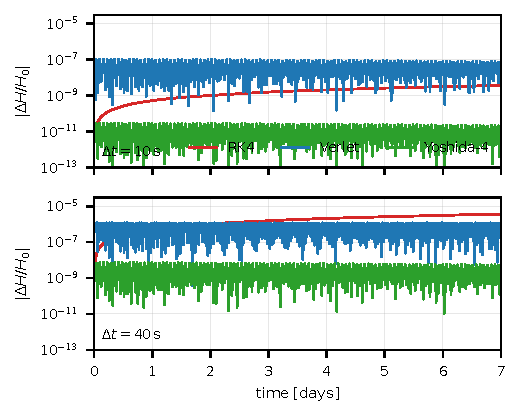
\includegraphics[width=\columnwidth]{fig1_drift}
\caption{7-day relative energy error, CPU, $\Delta t=10$\,s (top) and
$40$\,s (bottom). RK4 (dashed) grows secularly; Verlet and Yoshida-4 remain
bounded. Source: \texttt{paper/results/e1\_*\_7d.csv}.}
\label{fig:drift}
\end{figure}

\subsection{Reduction determinism and accuracy}
\label{sec:e2}
Figure~\ref{fig:reduce} summarizes all 9\,600 repeats. On the benign input,
FP64 accumulators sit at the summation floor ($1.2\times10^{-17}$ to
$3.6\times10^{-15}$ relative over all modes and sizes); FP32 errors
span $1.8\times10^{-9}$ to $7.4\times10^{-8}$ for the fixed and Kahan
trees and reach $3.0\times10^{-6}$ for atomic summation. The adversarial input
($\pm10^8$ with an $i \bmod 7$ residue) is an exact cliff: every FP32
summation---all three modes, all sizes, all 100 repeats---rounds to exactly
zero (relative error $1.0$), whereas FP64 partial sums stay integral below
$2^{53}$ and are bit-exact against the long-double oracle.

Repeatability is a mode property, not a platform accident
(Fig.~\ref{fig:reduce}c). Fixed-tree and Kahan reductions return exactly
one distinct value in 100 repeats at every $n$ and both accumulator
precisions. Atomic summation returns 2, 5, 13, and 42 distinct FP64 values
at $n=2^{16},2^{18},2^{20},2^{22}$ (28 at $2^{24}$), and 8--47 distinct
FP32 values at $n\ge2^{16}$---under one fixed launch configuration, so the variation comes
from device-side scheduling of atomic adds, not from our configuration
knobs. The cost of determinism is modest at $n=2^{20}$: 0.342\,ms fixed and
0.405\,ms Kahan versus 0.309\,ms atomic for an FP64 reduction (11\% and
31\% overhead).

\begin{figure}[t]
\centering
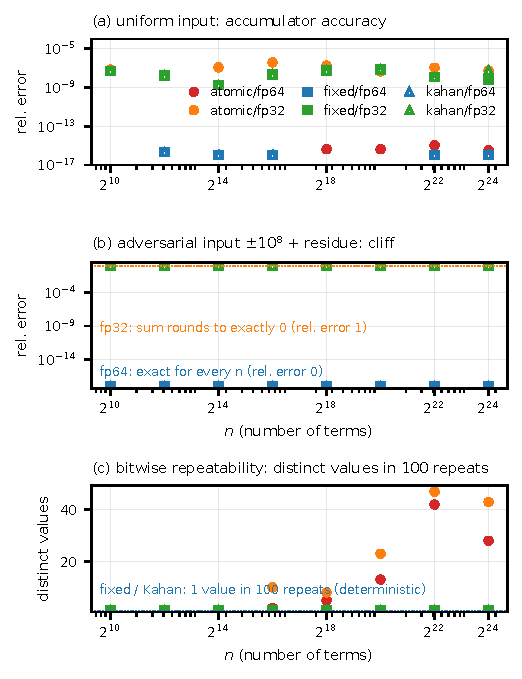
\includegraphics[width=\columnwidth]{fig2_reduce}
\caption{Reduction quality over 100 repeats. (a) Benign input accuracy
ladder; (b) adversarial cliff---FP32 collapses to a zero sum, FP64 stays
exact; (c) distinct results in 100 repeats---fixed/Kahan always one,
atomic varies with $n$. Source: \texttt{paper/results/e2\_reduce.csv}.}
\label{fig:reduce}
\end{figure}

\subsection{The FP32 noise floor}
\label{sec:e3}
Figure~\ref{fig:noise} overlays the first day of the 7-day ensemble
experiment. All three FP64 reduction modes and the long-double CPU
reference are indistinguishable: identical range
$[-5.18, +2.66]\times10^{-8}$, 100\% of samples nonzero. With FP32
accumulators the physics disappears into arithmetic. Summing
$H\approx-1.2\times10^{5}$ in FP32 has $\mathrm{ULP}=2^{-7}=7.8\times
10^{-3}$, i.e.\ a relative quantum of $6.49\times10^{-8}$---larger than the
oscillation itself. Fixed and Kahan FP32 tick at exactly that quantum
(range $\pm6.49\times10^{-8}$, 69\% of samples nonzero), and atomic FP32
pins a single value for the entire run (every sample identically zero
relative energy error). This is not a bug in the atomic path: no FP32
accumulator, in any mode, can represent the quantity being measured.

\begin{figure}[t]
\centering
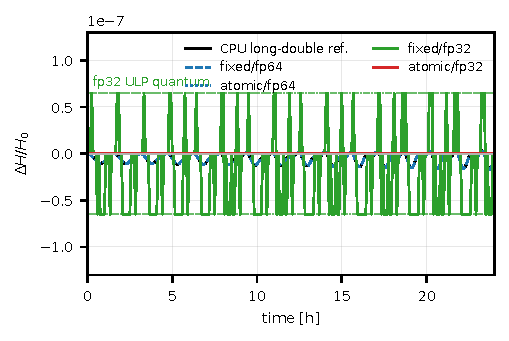
\includegraphics[width=\columnwidth]{fig3_noise}
\caption{First 24\,h of E3 ($n=4096$): FP64 modes track the CPU
reference; FP32 modes are quantized at the $\pm6.49\times10^{-8}$ ULP
quantum (dash-dot), with atomic FP32 flat at zero; Kahan FP32 is
bit-identical to fixed FP32 (not drawn). Source:
\texttt{paper/results/e3\_*.csv}.}
\label{fig:noise}
\end{figure}

\subsection{Accuracy-throughput Pareto}
\label{sec:e4}
Table~\ref{tab:e4} gives 7-day accuracy for the three state-precision
variants; Fig.~\ref{fig:pareto} places them against measured throughput.
FP64 GPU Verlet runs at 4.82\,ms/step versus 9.60\,ms for the 12-thread
CPU ($1.99\times$). FP32 state runs at 0.483\,ms ($9.98\times$ over GPU
FP64, $19.9\times$ over CPU) and the compensated variant at 0.724\,ms
($6.65\times$, $13.3\times$). The compensation earns its cost at every
time step: FP32k beats FP32 everywhere, by $4.2\times$ at $\Delta
t=10$\,s ($6.48\times10^{-6}$ vs.\ $2.72\times10^{-5}$). Note the honest
inversion of the classical rule for FP32: error \emph{falls} as
$\Delta t$ grows ($2.8\times10^{-5}$ at 5\,s to $6.7\times10^{-6}$ at
40\,s) because per-step rounding, not truncation, dominates at small
$\Delta t$. Figure~\ref{fig:pareto} shows the resulting bands: precision
sets the vertical position, state precision sets the horizontal one, and
FP32k occupies the useful corner.

\begin{table}[t]
\centering
\caption{Max $|\Delta H/H_0|$ over 7\,d, GPU Verlet (E4).}
\label{tab:e4}
\begin{tabular}{lcccc}
\hline
$\Delta t$ (s) & 5 & 10 & 20 & 40 \\
\hline
FP64  & $2.69\!\times\!10^{-8}$ & $1.04\!\times\!10^{-7}$ & $3.68\!\times\!10^{-7}$ & $1.18\!\times\!10^{-6}$ \\
FP32  & $2.80\!\times\!10^{-5}$ & $2.72\!\times\!10^{-5}$ & $2.09\!\times\!10^{-5}$ & $6.72\!\times\!10^{-6}$ \\
FP32k & $1.56\!\times\!10^{-5}$ & $6.48\!\times\!10^{-6}$ & $1.64\!\times\!10^{-5}$ & $4.40\!\times\!10^{-6}$ \\
\hline
\end{tabular}
\end{table}

\begin{figure}[t]
\centering
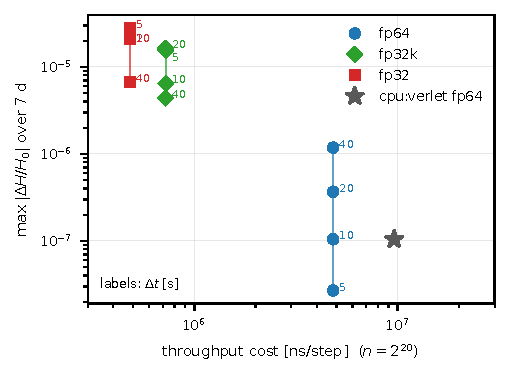
\includegraphics[width=\columnwidth]{fig4_pareto}
\caption{7-day max $|\Delta H/H_0|$ versus time per step
($n=2^{20}$, best of 5). Each precision forms a vertical band over
$\Delta t\in\{5,10,20,40\}$\,s; the star marks the 12-thread CPU. Source:
\texttt{paper/results/e4\_*.csv}.}
\label{fig:pareto}
\end{figure}

\section{Threats to Validity}
\label{sec:threats}

\textbf{Hardware generality.} All throughput numbers come from one
laptop Ampere GPU whose FP64 rate is $1/64$ FP32; on datacenter parts
(e.g.\ 1:2 rates) the FP32 speedups shrink substantially, while the
determinism and noise-floor results---properties of IEEE arithmetic and
reduction order---do not. \textbf{Model scope.} The engine models a
conservative field only; dissipative forces would change $H$ by design and
make this diagnostic meaningless, so conclusions apply to energy-conserving
settings. \textbf{Coverage.} One orbit regime (400\,km, 51.6$^\circ$),
$n\le2^{24}$, fixed-step integrators, and one device; atomic spread is
measured under a single launch configuration, and other GPUs or chunking
schemes will show different---but almost certainly nonzero---spread.
\textbf{Build.} No fast-math flags were used; results under
flush-to-zero modes or different compilers may shift FP32 floors by an
ULP or two, not their order of magnitude.

\section{Conclusion}
\label{sec:conclusion}

Noether's correspondence---symmetry, conservation, diagnostic---survives
parallel hardware only if the reduction that reports the conserved quantity
is treated as part of the algorithm, not as plumbing. Fixed-tree and Kahan
reductions restore bitwise determinism at 11--31\% overhead; atomic
summation does not, and its run-to-run spread varies with problem size.
FP32 accumulation is not a cheaper version of FP64: it changes what can be
measured at all, quantizing the symplectic oscillation into ULP steps and
collapsing under cancellation. The useful operating point on this hardware
is mixed precision: FP32 state with persistent kick compensation and FP64
energy evaluation buys $6.7\times$ GPU throughput at a bounded
$6.5\times10^{-6}$ error, leaving the structure of the flow---and the
diagnostic---intact.

\section*{Artifact Appendix}
\label{sec:artifact}

Everything is reproducible from a clean clone with three commands:
\begin{enumerate}
\item \texttt{cmake -S . -B build -DCMAKE\_BUILD\_TYPE=Release \&\&
      cmake --build build -j} \texttt{\&\&} \texttt{ctest --test-dir build
      --output-on-failure} (5/5 tests; CUDA tests skip without a device).
\item \texttt{./scripts/run\_experiments.sh} regenerates all 39 CSVs in
      \texttt{paper/results/} ($\sim$90\,s with a GPU).
\item \texttt{python3 analysis/fig1\_drift.py} (and \texttt{fig2},
      \texttt{fig3}, \texttt{fig4}) regenerates
      \texttt{paper/figs/*.pdf}; requirements in
      \texttt{analysis/requirements.txt}.
\end{enumerate}
Every number in this paper is computed from those CSVs by the figure
scripts or the commands shown in the captions. The paper itself builds with
\texttt{cd paper \&\& tectonic main.tex} (any \TeX\ toolchain with the
\texttt{newtx} fonts works).

\begin{thebibliography}{9}
\bibitem{verlet1967}
L.~Verlet, ``Molecular dynamics,'' \emph{Molecular Physics}, vol.~13,
pp.~197--199, 1967.

\bibitem{yoshida1990}
H.~Yoshida, ``Construction of higher order symplectic integrators,''
\emph{Physics Letters A}, vol.~150, pp.~262--268, 1990.

\bibitem{hairer2006}
E.~Hairer, C.~Lubich, and G.~Wanner, \emph{Geometric Numerical Integration:
Structure-Preserving Algorithms for Ordinary Differential Equations}, 2nd~ed.
Berlin: Springer, 2006.

\bibitem{kahan1965}
W.~Kahan, ``Further remarks on reducing truncation errors,'' \emph{Communications of the ACM}, vol.~8, p.~40, 1965.

\bibitem{higham2002}
N.~J.~Higham, \emph{Accuracy and Stability of Numerical Algorithms}, 2nd~ed.
Philadelphia: SIAM, 2002.

\bibitem{hoefler2015}
T.~Hoefler and A.~Belli, ``Scientific benchmarking of parallel computing
systems,'' in \emph{Proc. Int. Conf. High Performance Computing, Networking,
Storage and Analysis (SC)}, 2015, pp.~1--12.
\end{thebibliography}

\end{document}
